\documentclass[a4paper]{article}
\usepackage[utf8]{inputenc}
\usepackage[spanish, es-tabla]{babel}

\usepackage{amsmath}
\usepackage{amsfonts}
\usepackage{amssymb}

\usepackage{float}
\usepackage{graphicx}
\graphicspath{ {./Imagenes/} }

\usepackage[american voltage]{circuitikz}

\usepackage{fancyhdr}

\usepackage{units} 

\pagestyle{fancy}
\fancyhf{}
\lhead{22.02 Electrotecnia I}
\rhead{Mechoulam, Mestanza, Lambertucci, Pouthier, Londero}
\rfoot{Página \thepage}



\begin{document}

%%%%%%%%%%%%%%%%%%%%%%%%%%%%%%%%%%%%%%%%%%%%%%%%%%%%%%%%%%%%%%%%%%%%%%%%% 
%								CARATULA								%
%%%%%%%%%%%%%%%%%%%%%%%%%%%%%%%%%%%%%%%%%%%%%%%%%%%%%%%%%%%%%%%%%%%%%%%%% 

\begin{titlepage}
\newcommand{\HRule}{\rule{\linewidth}{0.5mm}}
\center
\mbox{\textsc{\LARGE \bfseries {Instituto Tecnológico de Buenos Aires}}}\\[1.5cm]
\textsc{\Large 22.02 Electrotecnia I}\\[0.5cm]


\HRule \\[0.6cm]
{ \Huge \bfseries Trabajo práctico N$^{\circ}$3}\\[0.4cm] 
\HRule \\[1.5cm]


{\large

\emph{Grupo 5}\\
\vspace{3px}

\begin{tabular}{lr} 	
\textsc{Mechoulam}, Alan  &  58438\\
\textsc{Lambertucci}, Guido Enrique  & 58009 \\
\textsc{Pouthier}, Florian  & 61337 \\
\textsc{Mestanza}, Nicolás  & 57521 \\
\textsc{Londero Bonaparte}, Tomás Guillermo  & 58150 \\
\end{tabular}

\vspace{20px}

\emph{Profesores}\\
\vspace{3px}
\textsc{Muñoz}, Claudio Marcelo\\ 	
\textsc{Ayub}, Gustavo\\ 	

\vspace{100px}

\begin{tabular}{ll}

Presentado: & 17/05/19\\

\end{tabular}

}

\vfill

\end{titlepage}


%%%%%%%%%%%%%%%%%%%%%%%%%%%%%%%%%%%%%%%%%%%%%%%%%%%%%%%%%%%%%%%%%%%%%%%%% 
%								INFORME									%
%%%%%%%%%%%%%%%%%%%%%%%%%%%%%%%%%%%%%%%%%%%%%%%%%%%%%%%%%%%%%%%%%%%%%%%%%

\section*{Introducción}

En el trabajo realizado se analizo el funcionamiento de un transformador. Se realizaron análisis en del circuito analizando las situaciones en corto, ne vacío y con carga. Para llevar adelante el experimento se utilizó:
\begin{itemize}
	\item[a)]	Ohmetro;
	\item[b)]	Voltímetro;
	\item[c)]	Amperímetro;
	\item[d)]	Vatímetro;
	\item[e)]	Inductancias; y
	\item[f)]	Autotransformador.
\end{itemize}

\section*{Desarrollo de la experiencia}

\section[I]{\underline{Primera parte}}

Para empezar se dispuso el circuito de la forma mostrada en la figura (\ref{fig:1a}). Luego, se colocó un voltímetro en los distintos bornes de las inductacias, de esta forma se buscó determinar de que manera serían homólogos, sabiendo que se daría dicha condición cuando la diferencia de tensión sea próxima a cero.

\begin{figure}[H]
	\centering
	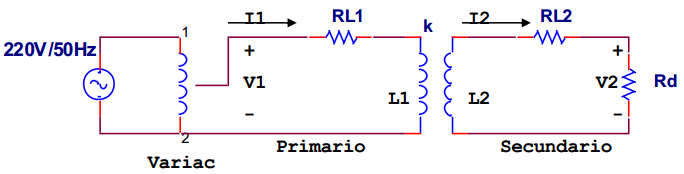
\includegraphics[width=0.8\textwidth]{Circuito-1.PNG}
	\caption{Circuito empleado.}
	\label{fig:1a}
\end{figure}

Así queda determinado el sentido de la inductancia mutua, conectando el circuito de forma tal que se vea de la forma mostrada en la figura

\begin{figure}[H]
\begin{center}
\begin{circuitikz}
	\draw
		
	(0.5,3)	to	[voltmeter] (3.5,3)

	(0,0)	to (1,0)
	%(0,1)	to (1,1)	
	(1,0)	node[transformer] {}
	
	(2,0)	node[circ]{}

	;\end{circuitikz}
\end{center}
\end{figure}


\section{\underline{Segunda parte}}

En esta parte, se va a hacer un análisis práctico de un transformador monofásico. El dicho es construido de la misma manera que antes con dos bobinas y un núcleo de hierro.

El objetivo es entonces de hallar los parámetros físicos de este transformador con diferentes ensayos sucesivos.

Con uno transformador de ese tipo, no se puede estimar rendimiento o regulación, porque ...

\subsection{Ensayo en vacío}

Para ese primer ensayo, se procede al armado del siguiente circuito :

\begin{circuitikz}
\draw
	(-1, -1.1) 		to [vL] (-1,-2.1)
	(-1.5, -1.1) 	to [short, *-] (-1, -1.1)
	(-1.5, -2.1) 	to [short, *-] (-1, -2.1)
					to (0,-2.1)
	(0,0)	to (0,-1.7)
			to (-0.6,-1.7)
	(0,0) 	to node[draw,circle,fill=white] {A} (1.5, 0)
			to node[draw,circle,fill=white] {W} (3.5, 0)
			to [short, -*] (5, 0) to (5.5,0)
	(0.7,0.7) node[]{$I_{10}$}
	(2.5,0.7) node[]{$P_{10}$}
	(2.5,-0.4) to (2.5,-2.1)
	(4,0) to node[draw,circle,fill=white] {V} (4, -2.1)
	(4.5,-0.5) node[]{$U_{10}$}
	(0,-2.1) to [short, -*] (5,-2.1) to (5.5,-2.1)
	(6.5,0) node[transformer core]{}
	(8,0) to (7,0) to [short, -*] (9.5,0)
	(8,-2.1) to (7,-2.1) to [short, -*] (9.5,-2.1)
	(8.5,0) to node[draw,circle,fill=white] {V} (8.5, -2.1)
	(9,-0.5) node[]{$U_{20}$};
\end{circuitikz}

Aplicando una tensión nominal cercana de 100 V, el vatímetro indicará las pérdidas en el hierro nominales.

\subsection{Ensayo en cortocircuito}

\subsection{Modelo resultante del transformador}

\end{document}
